\documentclass[14pt]{extbook}
\usepackage{multicol, enumerate, enumitem, hyperref, color, soul, setspace, parskip, fancyhdr} %General Packages
\usepackage{amssymb, amsthm, amsmath, latexsym, units, mathtools} %Math Packages
\everymath{\displaystyle} %All math in Display Style
% Packages with additional options
\usepackage[headsep=0.5cm,headheight=12pt, left=1 in,right= 1 in,top= 1 in,bottom= 1 in]{geometry}
\usepackage[usenames,dvipsnames]{xcolor}
\usepackage{dashrule}  % Package to use the command below to create lines between items
\newcommand{\litem}[1]{\item#1\hspace*{-1cm}\rule{\textwidth}{0.4pt}}
\pagestyle{fancy}
\lhead{Progress Quiz 3}
\chead{}
\rhead{Version A}
\lfoot{3012-8528}
\cfoot{}
\rfoot{Summer C 2021}
\begin{document}

\begin{enumerate}
\litem{
Find the equation of the line described below. Write the linear equation in the form $ y=mx+b $ and choose the intervals that contain $m$ and $b$.\[ \text{Perpendicular to } 3 x + 4 y = 15 \text{ and passing through the point } (8, 10). \]\begin{enumerate}[label=\Alph*.]
\item \( m \in [-1.82, -1.19] \hspace*{3mm} b \in [19.7, 22.4] \)
\item \( m \in [0.87, 1.78] \hspace*{3mm} b \in [-1.9, -0.6] \)
\item \( m \in [0.87, 1.78] \hspace*{3mm} b \in [-0.3, 1.1] \)
\item \( m \in [0.87, 1.78] \hspace*{3mm} b \in [1.9, 3] \)
\item \( m \in [-0.26, 0.92] \hspace*{3mm} b \in [-1.9, -0.6] \)

\end{enumerate} }
\litem{
Solve the equation below. Then, choose the interval that contains the solution.\[ -11(12x + 4) = -3(13x -5) \]\begin{enumerate}[label=\Alph*.]
\item \( x \in [-0.96, -0.63] \)
\item \( x \in [-0.1, 0.58] \)
\item \( x \in [-0.28, -0.02] \)
\item \( x \in [-0.61, -0.2] \)
\item \( \text{There are no real solutions.} \)

\end{enumerate} }
\litem{
Write the equation of the line in the graph below in Standard Form $Ax+By=C$. Then, choose the intervals that contain $A, B, \text{ and } C$.
\begin{center}
    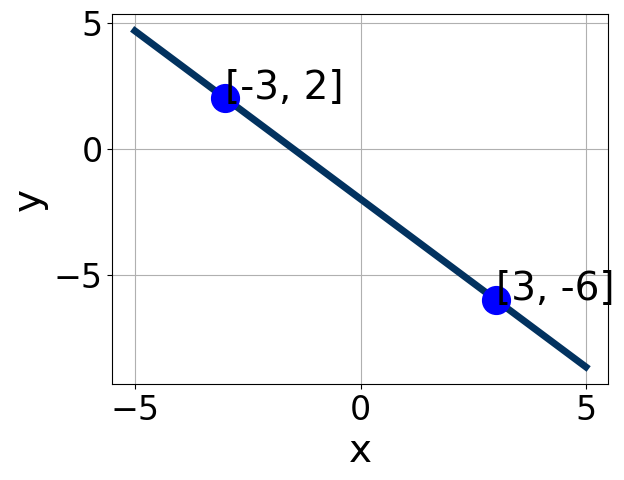
\includegraphics[width=0.5\textwidth]{../Figures/linearGraphToStandardCopyA.png}
\end{center}
\begin{enumerate}[label=\Alph*.]
\item \( A \in [2, 6], \hspace{3mm} B \in [2.44, 4.14], \text{ and } \hspace{3mm} C \in [-6.2, -4.4] \)
\item \( A \in [-8, -2], \hspace{3mm} B \in [-4.02, -2.76], \text{ and } \hspace{3mm} C \in [2.9, 8] \)
\item \( A \in [-2.67, 3.33], \hspace{3mm} B \in [0.8, 2.59], \text{ and } \hspace{3mm} C \in [-4.7, -0.7] \)
\item \( A \in [2, 6], \hspace{3mm} B \in [-4.02, -2.76], \text{ and } \hspace{3mm} C \in [2.9, 8] \)
\item \( A \in [-2.67, 3.33], \hspace{3mm} B \in [-1.55, -0.2], \text{ and } \hspace{3mm} C \in [0.4, 5] \)

\end{enumerate} }
\litem{
Find the equation of the line described below. Write the linear equation in the form $ y=mx+b $ and choose the intervals that contain $m$ and $b$.\[ \text{Parallel to } 9 x + 4 y = 10 \text{ and passing through the point } (6, -8). \]\begin{enumerate}[label=\Alph*.]
\item \( m \in [-4.25, -1.25] \hspace*{3mm} b \in [-5.5, -3.5] \)
\item \( m \in [-4.25, -1.25] \hspace*{3mm} b \in [0.5, 9.5] \)
\item \( m \in [0.25, 4.25] \hspace*{3mm} b \in [-21.5, -18.5] \)
\item \( m \in [-4.25, -1.25] \hspace*{3mm} b \in [-16, -8] \)
\item \( m \in [-1.44, 0.56] \hspace*{3mm} b \in [0.5, 9.5] \)

\end{enumerate} }
\litem{
Write the equation of the line in the graph below in Standard Form $Ax+By=C$. Then, choose the intervals that contain $A, B, \text{ and } C$.
\begin{center}
    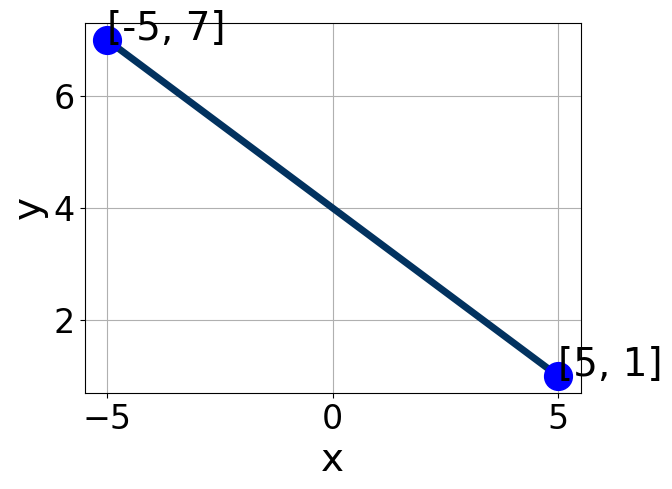
\includegraphics[width=0.5\textwidth]{../Figures/linearGraphToStandardA.png}
\end{center}
\begin{enumerate}[label=\Alph*.]
\item \( A \in [-6, -2], \hspace{3mm} B \in [-6.5, -4.1], \text{ and } \hspace{3mm} C \in [-21, -19] \)
\item \( A \in [1, 4], \hspace{3mm} B \in [-6.5, -4.1], \text{ and } \hspace{3mm} C \in [-21, -19] \)
\item \( A \in [-2.4, 2.6], \hspace{3mm} B \in [-4.5, -0.6], \text{ and } \hspace{3mm} C \in [-6, -2] \)
\item \( A \in [-2.4, 2.6], \hspace{3mm} B \in [0.5, 2.9], \text{ and } \hspace{3mm} C \in [1, 9] \)
\item \( A \in [1, 4], \hspace{3mm} B \in [3.5, 5.3], \text{ and } \hspace{3mm} C \in [19, 21] \)

\end{enumerate} }
\litem{
Solve the linear equation below. Then, choose the interval that contains the solution.\[ \frac{3x -4}{4} - \frac{5x + 6}{2} = \frac{-7x -8}{3} \]\begin{enumerate}[label=\Alph*.]
\item \( x \in [-0.2, 1.5] \)
\item \( x \in [-8.5, -6.8] \)
\item \( x \in [0.3, 3] \)
\item \( x \in [2.9, 5.1] \)
\item \( \text{There are no real solutions.} \)

\end{enumerate} }
\litem{
First, find the equation of the line containing the two points below. Then, write the equation in the form $ y=mx+b $ and choose the intervals that contain $m$ and $b$.\[ (-4, -8) \text{ and } (7, -5) \]\begin{enumerate}[label=\Alph*.]
\item \( m \in [-1.69, -0.19] \hspace*{3mm} b \in [-3.48, -3.05] \)
\item \( m \in [0.25, 0.35] \hspace*{3mm} b \in [-4.26, -3.91] \)
\item \( m \in [0.25, 0.35] \hspace*{3mm} b \in [-13.01, -11.52] \)
\item \( m \in [0.25, 0.35] \hspace*{3mm} b \in [5.35, 7.65] \)
\item \( m \in [0.25, 0.35] \hspace*{3mm} b \in [-8.14, -6.21] \)

\end{enumerate} }
\litem{
Solve the linear equation below. Then, choose the interval that contains the solution.\[ \frac{4x -5}{8} - \frac{7x -8}{5} = \frac{-4x + 7}{3} \]\begin{enumerate}[label=\Alph*.]
\item \( x \in [3.1, 3.26] \)
\item \( x \in [8.68, 9.71] \)
\item \( x \in [0.88, 1.5] \)
\item \( x \in [10.29, 11.53] \)
\item \( \text{There are no real solutions.} \)

\end{enumerate} }
\litem{
Solve the equation below. Then, choose the interval that contains the solution.\[ -16(6x -13) = -10(-4x -3) \]\begin{enumerate}[label=\Alph*.]
\item \( x \in [1.32, 2.57] \)
\item \( x \in [-1.84, -1.38] \)
\item \( x \in [3.37, 4.88] \)
\item \( x \in [1.2, 1.37] \)
\item \( \text{There are no real solutions.} \)

\end{enumerate} }
\litem{
First, find the equation of the line containing the two points below. Then, write the equation in the form $ y=mx+b $ and choose the intervals that contain $m$ and $b$.\[ (9, 2) \text{ and } (4, -4) \]\begin{enumerate}[label=\Alph*.]
\item \( m \in [0.2, 4.2] \hspace*{3mm} b \in [-9.72, -8.07] \)
\item \( m \in [0.2, 4.2] \hspace*{3mm} b \in [-7.07, -6.82] \)
\item \( m \in [-6.2, 0.8] \hspace*{3mm} b \in [0.18, 1.12] \)
\item \( m \in [0.2, 4.2] \hspace*{3mm} b \in [8.48, 10.02] \)
\item \( m \in [0.2, 4.2] \hspace*{3mm} b \in [-8.74, -7.05] \)

\end{enumerate} }
\end{enumerate}

\end{document}